\documentclass[aps,prl,reprint,nobalancelastpage,nofootinbib]{revtex4-2}
\usepackage[utf8]{inputenc}
\usepackage{amsmath}
\usepackage{amssymb}
\usepackage{tikz}
\usetikzlibrary{calc}
\usepackage{xcolor}
\usepackage[framemethod=tikz]{mdframed}

\begin{document}

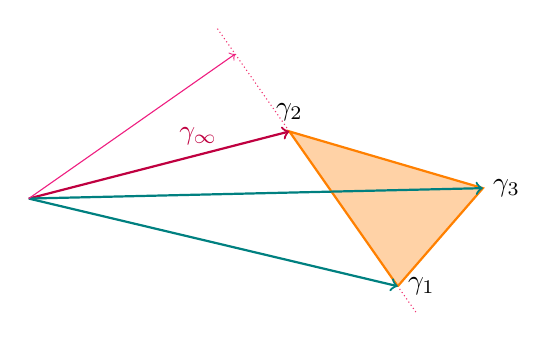
\begin{tikzpicture}[xscale=0.80,yscale=0.80,every node/.style={font=\normalsize},rotate=35]

\draw[densely dotted, magenta!65!orange] (4,-5) -- (4,0.5);
\draw[orange, thick, fill=orange!35!white] (4,-4.5) -- (4,-1.5) -- (6,-4) -- (4,-4.5);

\draw[->, thick, teal] (0,0) -- (4,-4.5) node[right,black]{$\gamma_1$};
\draw[->, thick, purple] (0,0) -- (4,-1.5) node[above,black]{$\gamma_2$} node[above, pos=0.65] {$\gamma_\infty$};
\draw[->, thick, teal] (0,0) -- (6,-4) node[right,black]{$\gamma_3$};

\draw[->, magenta!80!orange] (0,0) -- (4,0);

\end{tikzpicture}

\end{document}